
%%%%%%%%%%%%%%%%%%%%%%%%%%%%%%%%%%%%%%%%%%%%%%%%%%%%%%%%%%%%%%%%%%%%%%%%%%
\begin{figure} \centering {\setlength{\unitlength}{1.0in}
\begin{picture}(6.500,1.600)(0,0.05)

   \put(0.00,0.00){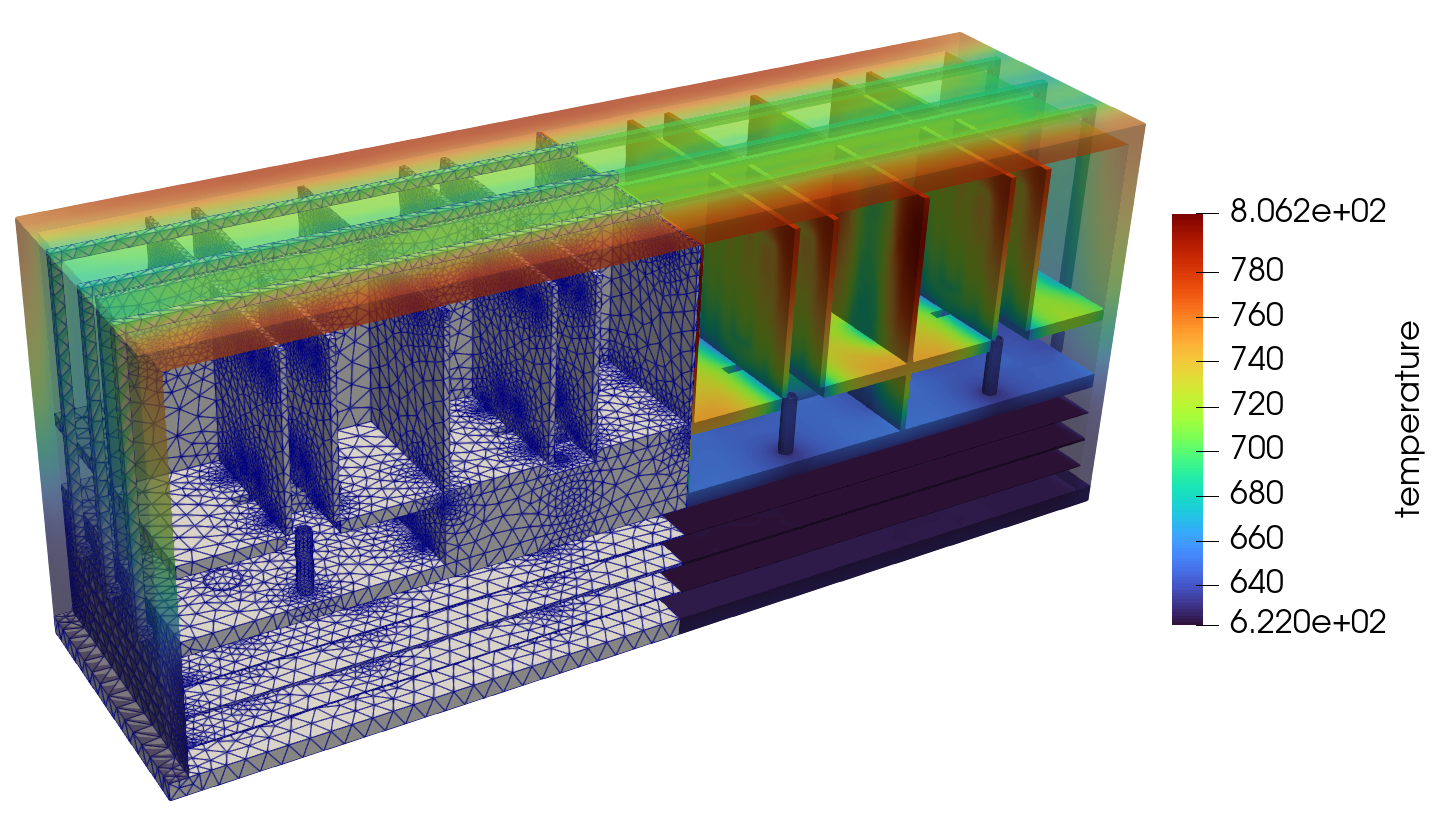
\includegraphics[width=2.80in]{figures/temp_mesh.png}}
   \put(0.20,1.50){(a)}

   \put(3.10,0.00){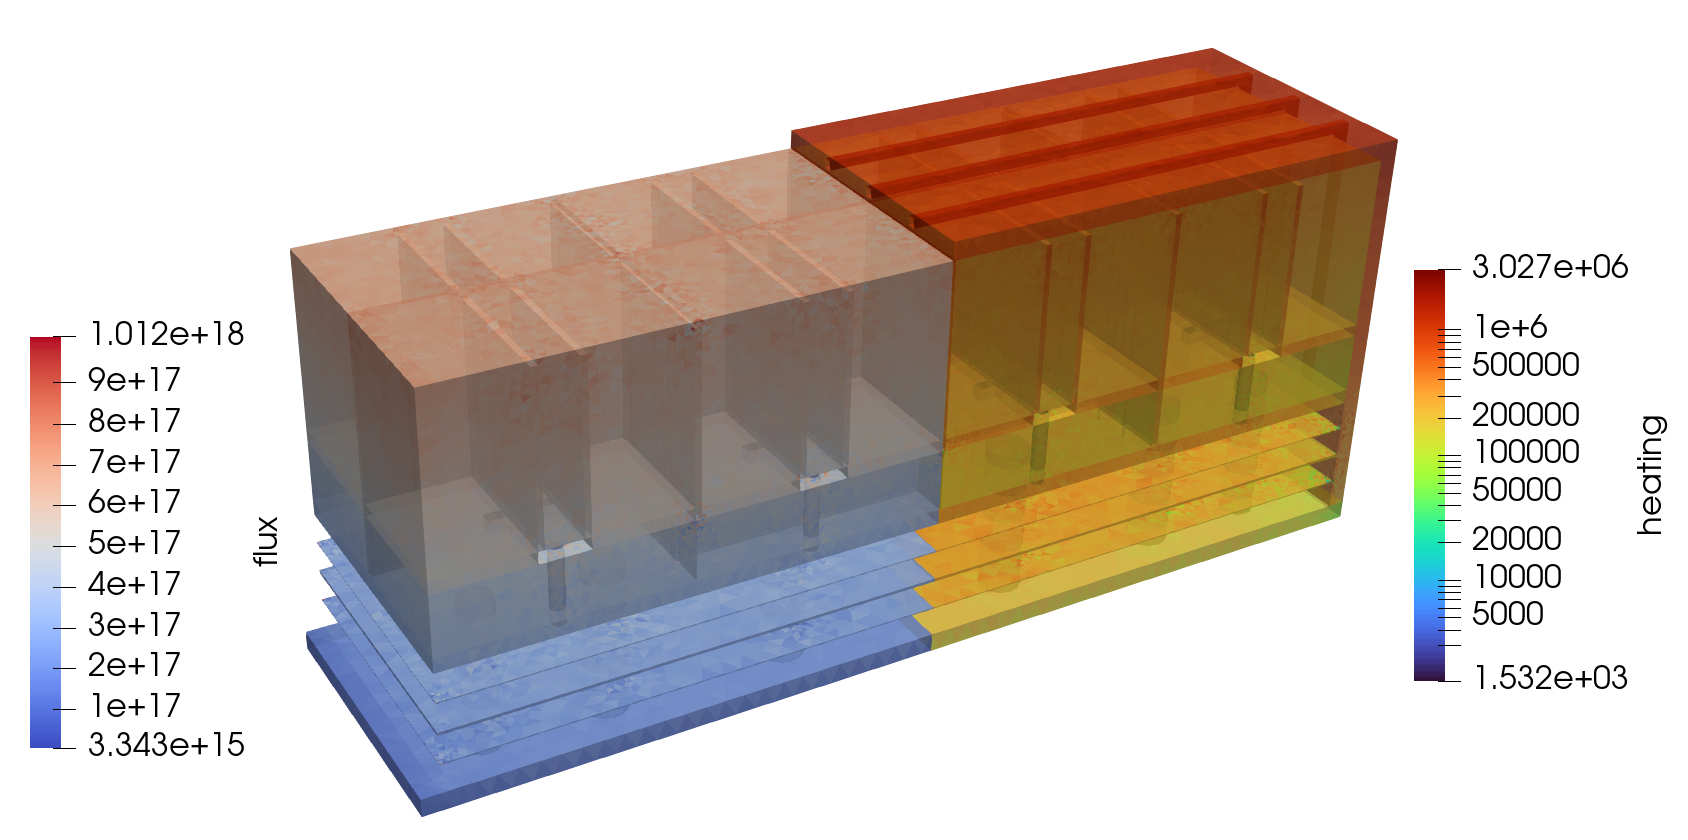
\includegraphics[width=3.40in]{figures/flux_heating.png}}
   \put(3.47,1.50){(b)}

\end{picture}}
\caption{\label{fig:fc}\small 
(a) Solid temperature computed using MOOSE, coupled to OpenMC radiation transport.
(b) OpenMC neutron flux (left) and energy deposition (right), coupled to MOOSE heat conduction.
} 
\end{figure}
%%%%%%%%%%%%%%%%%%%%%%%%%%%%%%%%%%%%%%%%%%%%%%%%%%%%%%%%%%%%%%%%%%%%%%%%%%

In Year 1, we established baseline simulations for a single breeder module (Task BB.I) on Frontier, focusing on the HCLL blanket from the EU DEMO. Radiation transport was modeled in OpenMC using Monte Carlo methods on DAGMC-generated geometry; heat conduction was solved in MOOSE on a tetrahedral mesh. The parametric CAD model enables rapid design changes. Coupling was achieved via Cardinal, embedding OpenMC within MOOSE and enabling data transfer between bases using nearest-element mapping. MOOSE used distributed mesh parallelism; OpenMC did not. Frontier runs helped determine suitable mesh resolutions for standalone and coupled cases. Figure~\ref{fig:fc} shows (a) solid temperature from MOOSE and (b) OpenMC neutron flux and energy deposition.  TBR is a critical fusion metric. To assess geometry evolution effects, we developed a novel moving mesh feature in Cardinal, enabling OpenMC to track particles on time-varying MOOSE meshes. Verified against benchmarks, this will support Year 2 studies on structural effects on TBR.


